%%%%%%%%%%%%%%%%%%%%%%%%%%%%%%%%%%%%%%%%%
% Academic Title Page
% LaTeX Template
% Version 2.0 (17/7/17)
%
% This template was downloaded from:
% http://www.LaTeXTemplates.com
%
% Original author:
% WikiBooks (LaTeX - Title Creation) with modifications by:
% Vel (vel@latextemplates.com)
%
% License:
% CC BY-NC-SA 3.0 (http://creativecommons.org/licenses/by-nc-sa/3.0/)
% 
% Instructions for using this template:
% This title page is capable of being compiled as is. This is not useful for 
% including it in another document. To do this, you have two options: 
%
% 1) Copy/paste everything between \begin{document} and \end{document} 
% starting at \begin{titlepage} and paste this into another LaTeX file where you 
% want your title page.
% OR
% 2) Remove everything outside the \begin{titlepage} and \end{titlepage}, rename
% this file and move it to the same directory as the LaTeX file you wish to add it to. 
% Then add \input{./<new filename>.tex} to your LaTeX file where you want your
% title page.
%
%%%%%%%%%%%%%%%%%%%%%%%%%%%%%%%%%%%%%%%%%

%----------------------------------------------------------------------------------------
%	PACKAGES AND OTHER DOCUMENT CONFIGURATIONS
%----------------------------------------------------------------------------------------

\documentclass[11pt]{article}

\usepackage[utf8]{inputenc} % Required for inputting international characters
\usepackage[T1]{fontenc} % Output font encoding for international characters
\usepackage{mathpazo} % Palatino font
\usepackage{hyperref}
\usepackage{graphicx}
\usepackage{float}

\renewcommand*\contentsname{Obsah}

\begin{document}

%----------------------------------------------------------------------------------------
%	TITLE PAGE
%----------------------------------------------------------------------------------------

\begin{titlepage} % Suppresses displaying the page number on the title page and the subsequent page counts as page 1
	\newcommand{\HRule}{\rule{\linewidth}{0.5mm}} % Defines a new command for horizontal lines, change thickness here
	
	\center % Centre everything on the page
	
	%------------------------------------------------
	%	Headings
	%------------------------------------------------
	
	\textsc{\LARGE Slovenská Technická Univerzita}\\[1.5cm] % Main heading such as the name of your university/college
	
	\textsc{\Large Fakulta informatiky a informačných technológií}\\[0.5cm] % Major heading such as course name
	
	\textsc{\large Mobilné technológie a aplikácie}\\[0.5cm] % Minor heading such as course title
	
	%------------------------------------------------
	%	Title
	%------------------------------------------------
	
	\HRule\\[0.4cm]
	
	{\huge\bfseries SIP Proxy (telefónna ústredňa)}\\[0.4cm] % Title of your document
	
	\HRule\\[1.5cm]
	
	%------------------------------------------------
	%	Author(s)
	%------------------------------------------------
	
	\begin{minipage}{0.4\textwidth}
		\begin{flushleft}
			\large
			\textit{Autor}\\
			\textsc{Jakub Smorada} % Your name
		\end{flushleft}
	\end{minipage}
	~
	\begin{minipage}{0.4\textwidth}
		\begin{flushright}
			\large
			\textit{Cvičiaci}\\
			\textsc{Ing. Marek Galinski, PhD.} % Supervisor's name
		\end{flushright}
	\end{minipage}
	
	% If you don't want a supervisor, uncomment the two lines below and comment the code above
	%{\large\textit{Author}}\\
	%John \textsc{Smith} % Your name
	
	%------------------------------------------------
	%	Date
	%------------------------------------------------
	
	\vfill\vfill\vfill % Position the date 3/4 down the remaining page
	
	{\large27. február 2022} % Date, change the \today to a set date if you want to be precise
	
	%------------------------------------------------
	%	Logo
	%------------------------------------------------
	
	%\vfill\vfill
	%\includegraphics[width=0.2\textwidth]{placeholder.jpg}\\[1cm] % Include a department/university logo - this will require the graphicx package
	 
	%----------------------------------------------------------------------------------------
	
	\vfill % Push the date up 1/4 of the remaining page

\end{titlepage}

%----------------------------------------------------------------------------------------
\newpage
\tableofcontents
\newpage
\section{Zadanie úlohy}

\subsection{Hlavná myšlienka zadania}
Na vašom počítači (alebo virtuálnom počítači) sprevádzkujte SIP Proxy, ktorá umožní prepájanie a realizáciu hovorov medzi štandardnými SIP klientami.

\subsection{Doplňujúce informácie k zadaniu}
Na implementáciu vašej SIP Proxy si môžete zvoliť akýkoľvek programovací jazyk a použiť akúkoľvek SIP knižnicu, ktorá pre daný programovací jazyk existuje. Vo výsledku však musíte spúšťať “váš kód”, v ktorom sú zakomponované knižnice, ktoré poskytujú funkcionalitu SIP Proxy. To znamená, že nemôžete zobrať existujúcu SIP Proxy ako napr. Asterisk, kde len skompilujete alebo priamo spustíte cudziu binárku... Hovor musí byť realizovaný medzi dvomi fyzickými zariadeniami v rámci LAN siete.

\subsection{Rozsah povinných funkcionalít}

\begin{itemize}
	\item Registrácia účastníka (bez nutnosti autentifikácie)
	\item Vytočenie hovoru a zvonenie na druhej strane
	\item Prijatie hovoru druhou stranou, fungujúci hlasový hovor
	\item Ukončenie hlasového hovoru (prijatého aj neprijatého)
\end{itemize}

Ak sú splnené všetky tieto podmienky, študent získava 5 bodov, ktoré sú minimom na absolvovanie tohoto zadania.

\subsection{Doplnkové funkcionality (ktoré môžete, ale nemusíte urobiť)}

\begin{itemize}
	\item Možnosť zrealizovať konferenčný hovor (aspoň 3 účastníci)
	\item Možnosť presmerovať hovor
	\item Možnosť realizovať videohovor
	\item Logovanie “denníka hovorov” – kto kedy komu volal, kedy bol ktorý hovor prijatý, kedy bol ktorý hovor ukončený, do ľubovoľného textového súboru v ľubovoľnom formáte
	\item Úprava SIP stavových kódov z zdrojovom kóde proxy, napr. “486 Busy Here” zmeníte na “486
	Obsadené”
\end{itemize}

Každá doplnková funkcionalita predstavuje plus 1 bod.
Počas prezentácie zadania musíte byť schopní na zariadení, kde beží ústredňa urobiť SIP trace a otvoriť ho pomocou tcpdump alebo Wireshark, a v primeranom rozsahu vysvetliť cvičiacemu, ako daná signalizácia prebieha.

\section{Moja implementácia}

Pre moju implementáciu tohto zadania som využíval knižnicu z nasledujúceho repozitára: \url{https://github.com/tirfil/PySipFullProxy}. 
\\Odkaz na môj repozitár: \url{https://github.com/JakubSmorada/fiit_mtaa}.
\
\subsection{Povinné funkcionality}
\subsubsection{Registrácia účastníka}

Predtým než bude možné uskutočňovať hovory medzi účastníkmi, je potrebné aby sa zaregistrovali na SIP proxy server. Registrácia účastníka prebieha tak, že účastník na proxy server pošle požiadavku (request) REGISTER bez nutnosti autentifikácie. Server (pri korektnom správaní) následne posiela správu 200 OK (ako odpoveď na požiadavku REGISTER) a týmto je účastník zaregistrovaný.

\subsubsection{Vytočenie hovoru a zvonenie na druhej strane}

Po zaregistrovaní dvoch (alebo viacerích) účastníkov je teraz možné medzi nimi realizovať hovory. Nazvime týchto dvoch účastníkov Alice a Bob. Obaja z účastníkov musia mať unikátnu IP adresu z rovnakej siete. Alice sa snaží zavolať Bobovi na telefón. Alice (jej zariadenie) posiela na proxy server požiadavku INVITE. Proxy server tento kód preposiela Bobovi. Bob teraz posiela Alice cez proxy server jeho stav 100 Trying. Následne Bob posiela stavovy kód 180 Ringing, to znamená, že Bobove zariadenie už začalo zvoniť. 

\subsubsection{Prijatie hovoru druhou stranou, fungujúci hlasový hovor}

Pokračujme v predošlom scenári. Po tom čo Bob zdvihol hovor, jeho zariadenie posiela cez proxy server Alice správu 200 OK. Alice po prijatí tejto správy pošle naspäť ešte ACK, aby potvrdila prijatie správy. Teraz sa už začína hovor. SIP z angl. Session Initiation Protocol slúži iba na prepájanie hovorov a teda pri prebiehajúcom hovore už SIP proxy server nie je potrebný. Na samotné spracovanie hovoru, teda posielanie hlasu alebo videa druhej strane, slúži protokol RTP (Real-Time Protocol). RTP teda nepotrebuje prostredníka, dáta posiela priamo druhému účastníkovi hovoru.

\subsubsection{Ukončenie hlasového hovoru (prijatého aj neprijatého)}

Pri ukončení hovora vysiela ten účastník, ktorý chce hovor ukončiť požiadavku BYE druhému účastníkovi hovoru cez proxy server. Druhý účastník odpovedá na túto požiadavku (cez proxy server) stavovym kódom 200 OK, čím sa ukončí hovor.

\subsection{Doplnkové funkcionality}

\subsubsection{Možnosť zrealizovať konferenčný hovor, možnosť presmerovať hovor a možnosť realizovať videohovor}

Tieto 3 doplnkové funkcie sú už priamo zabezpečené prostredníctvom VoIP klienta Linphone, ktorý som využíval pri testovaní mojej implementácie. Všetky scenáre týchto doplnkových funkcií sú zobrazené v PCAP súboroch na mojom githube.

\subsubsection{Logovanie “denníka hovorov”}
V mojom riešení problému som logovanie denníka hovorov neimplementoval.

\subsubsection{Úprava SIP stavových kódov v zdrojovom kóde proxy}
V mojej implementácii som zmenil stavové kódy 100 Trying na 100 Skusam, 180 Ringing na 180 Zvonim a 486 Busy here na 486 Obsadene. V nasledujúcom obrázku je vidieť, ako sa na proxy serveri menia stavové kódy a následne posielajú ďalej na klienta.
\begin{figure}[H]
	\centering
	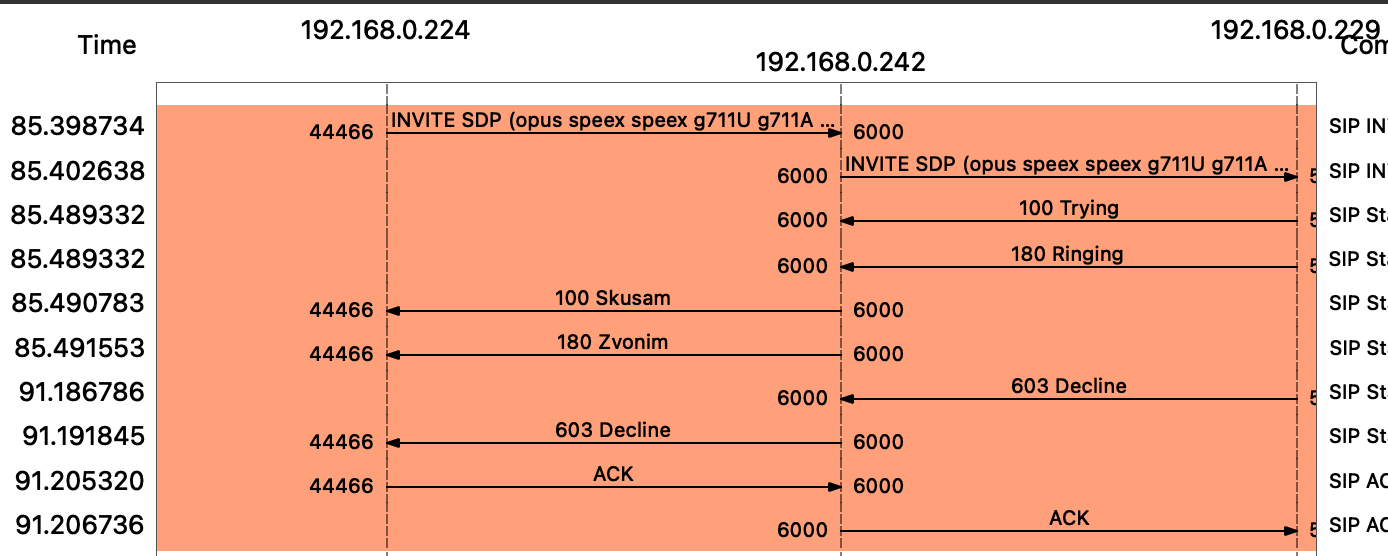
\includegraphics[width=1\textwidth]{stavove_kody.png}
	\caption{Úprava stavových kódov}
\end{figure}

\section{Záver}
Toto zadanie mi dalo prehľad o tom ako funguje VoIP a ako sa dokáže presúvať hlas a video cez IP sieť. Zároveň by som podotkol, že lepšou alternatívou by bolo spojazdnenie SIP proxy servera bez pomoci nejakej knižnice, s tým, že by sme na to mali viac času.


\end{document}
